\begin{figure}[htbp]
\centering
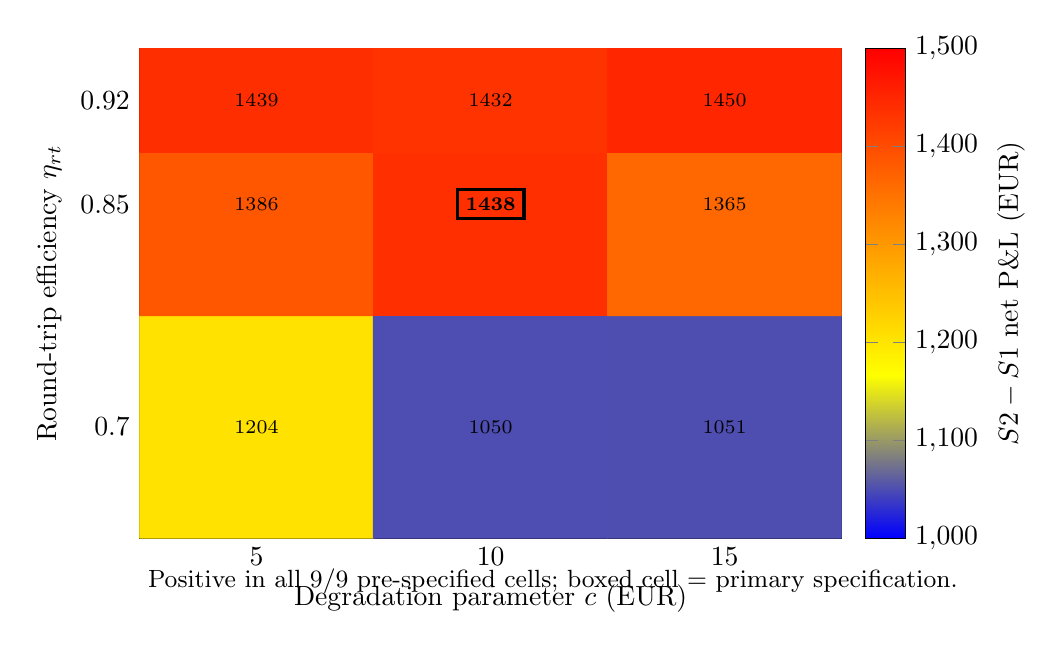
\begin{tikzpicture}
\begin{axis}[
  width=10.5cm,
  height=7.8cm,
  view={0}{90},
  xlabel={Degradation parameter \(c\) (EUR)},
  ylabel={Round-trip efficiency \(\eta_{rt}\)},
  xtick={5,10,15},
  ytick={0.70,0.85,0.92},
  point meta min=1000,
  point meta max=1500,
  colorbar,
  colorbar style={ylabel={\(S2-S1\) net P\&L (EUR)}},
  enlargelimits=false
]
\addplot[
  matrix plot*,
  mesh/cols=3,
  point meta=explicit
] coordinates {
(5,0.70) [1204.4233] (10,0.70) [1050.0490] (15,0.70) [1050.9575]
(5,0.85) [1386.1369] (10,0.85) [1437.5964] (15,0.85) [1364.7305]
(5,0.92) [1439.2135] (10,0.92) [1432.4232] (15,0.92) [1449.8080]
};
% cell annotations
\node at (axis cs:5,0.70) {\scriptsize 1204};
\node at (axis cs:10,0.70) {\scriptsize 1050};
\node at (axis cs:15,0.70) {\scriptsize 1051};
\node at (axis cs:5,0.85) {\scriptsize 1386};
\node[draw,very thick,inner sep=3pt] at (axis cs:10,0.85) {\scriptsize \textbf{1438}};
\node at (axis cs:15,0.85) {\scriptsize 1365};
\node at (axis cs:5,0.92) {\scriptsize 1439};
\node at (axis cs:10,0.92) {\scriptsize 1432};
\node at (axis cs:15,0.92) {\scriptsize 1450};
\end{axis}
\node[font=\small] at (5.25,-0.55) {Positive in all 9/9 pre-specified cells; boxed cell = primary specification.};
\end{tikzpicture}
\caption{Sensitivity of the holdout forecast-value contrast \(S2-S1\) across the pre-specified efficiency and degradation-cost grid. Every cell is positive; the boxed cell is the primary setting \((\eta_{rt}=0.85,c=10)\).}
\label{fig:sensitivity_heatmap}
\end{figure}
